\documentclass[12pt]{article} % The document class with options

\usepackage[margin=1in]{geometry}
\usepackage[utf8]{inputenc} 
\geometry{a4paper}
\usepackage{newtxtext,newtxmath}
\usepackage[T1]{fontenc}
\usepackage{amsmath}
\usepackage{amsfonts}
\usepackage{microtype}
\usepackage{graphicx}
\usepackage{listings} % For formatting and highlighting code
\usepackage{color}    % For colors in code highlighting

% chktex-file 2
% chktex-file 3
% chktex-file 8
% chktex-file 10
% chktex-file 17
% chktex-file 18
% chktex-file 36
% chktex-file 44

\begin{document}
\setlength{\parskip}{1em} 
\setlength{\parindent}{0pt}
\newcommand{\vect}[1]{\mathbf{#1}}

\begin{titlepage}  % This starts a title page environment
    \centering    % Center everything on the page

    %--- Add space at the top of the page ---
    \vspace*{2cm}
    
    %--- Title ---
    \normalsize \textbf{MEng Project Report} \\
    \vspace{0.5cm}  % Space between lines
    \normalsize\textbf{Global Response of Ship Models under the Influence of Surface Waves} \\
    \vspace{2cm}  % Space between the title and the author name
    
    %--- Author ---
    \normalsize by\\
    \vspace{1cm}
    \normalsize Jincong Li \\ 
    \vspace{1cm}
    \normalsize M.Eng, The University of British Columbia, 2024
    \vspace{11cm}  % Space between the author and the date
    
    %--- Date ---
    \normalsize \today

    \vfill  % Push the following content to the bottom of the page
    %--- Bottom part of the page ---
    © Jincong Li, 2024
\end{titlepage}
\tableofcontents
\newpage
\section{Abstract}

\section{Introduction}
This work is a branch of study in Near-Field Noise from Hull and Propeller (HARP). 
The HARP project focuses on the identification, characterization, and propagation of sound sources, 
which involve highly nonlinear multiphysics and multiscale physics. This research encompasses both 
near-field and far-field effects, with a particular emphasis on the following areas:

\begin{itemize}
    \item \textbf{Generation:} Investigation of near-field hull and propeller fluid-structure 
    interaction physics, including bubble wake flows and bubble-wall interactions.
    \item \textbf{Radiation:} Analysis of the far-field effects of the complex dynamical ocean 
    environment, considering factors such as turbulence, waves, currents, temperature, and salinity.
\end{itemize}

Additionally, the project aims to enhance the physical understanding and mitigation of underwater 
noise through:

\begin{itemize}
    \item Evaluating frequency, volume, duration, and the time to reach maximum noise levels.
    \item Developing monitoring and mitigation techniques, technologies, and methods, such as 
    optimizing ship speed and propeller pitch, and designing bio-inspired propeller blades and hulls.
\end{itemize}

This comprehensive approach aims to contribute to quieter and more efficient ship designs, 
balancing environmental performance with operational efficacy.

Underwater radiated noise (URN) sources comes from:
\begin{enumerate}
    \item vortex created by hull forms and appendages
    \item structure vibration creating pressure waves
    \item gear mesh
    \item propeller crating pressure waves
\end{enumerate}
Thus, as a branch of the HARP project, this work investigated into the global response/vibration 
of ship models under the influence of surface waves. 




\newpage
\section{Methodology}
The primary workflow of this project involves a two-step process. The initial step is to reproduce 
the results from Section 9.2 of Vaibhav Joshi's Ph.D. thesis\cite{joshi2018}. This section focuses 
on the analysis of the DTMB5415 ship model. The subsequent step is to replace the DTMB5415 ship model 
with the BURNSi ship model and conduct a similar model analysis.

The main target of this analysis is to study the heave motion of the BURNSi ship model under the 
same inlet wave conditions as those described in Section 9.2 of \cite{joshi2018}. By maintaining 
consistent wave conditions, we aim to directly compare the performance and characteristics of the 
BURNSi ship model against the baseline results obtained from the DTMB5415 ship model.

\begin{enumerate}
    \item \textbf{Reproduce Section 9.2 Results:}
    \begin{itemize}
        \item Follow the methodology outlined in Vaibhav Joshi's thesis to recreate the results 
        using the DTMB5415 ship model.
        \item Validate the accuracy and consistency of the reproduced results with the original 
        findings.
    \end{itemize}
    \item \textbf{Model Analysis with BURNSi Ship Model:}
    \begin{itemize}
        \item Replace the DTMB5415 ship model with the BURNSi ship model in the simulation framework.
        \item Conduct a detailed analysis focusing on the heave motion of the BURNSi ship model.
        \item Utilize the same inlet wave conditions as specified in Section 9.2 of \cite{joshi2018} 
        to ensure comparability.
    \end{itemize}
\end{enumerate}

This approach allows for a systematic evaluation of the BURNSi ship model's performance in terms of 
its heave motion response, providing valuable insights for further improvements and applications.
%The main workflow of this project is first reproduce the result from section 9.2 of the Vaibhav's Ph.D thesis\cite{joshi2018}. 
%Then replace the DTMB5415 ship model with the BURNSi ship model to conduct a model analysis of that ship. The main target is the
%heave motion of the BURNSi ship model under the same inlet wave conditions as in the section 9.2 of\cite{joshi2018}.
\subsection{DTMB5415}

The ship model used for the first part of this project is David Taylor Model
Basin (DTMB5415) as shwon in figure 1, which was conceived as a preliminary design for a Navy surface 
combatant around 1980. The hull geometry of Model 5415 includes both a sonar dome and a transom stern. Propulsion is provided through twin open-water propellers driven by shafts supported by struts.

It is important to note that no full-scale ship exists for this model. The hull geometry and relevant 
loading conditions and speeds are detailed below and in the Appendix section.
\begin{figure}[ht]
    \centering
    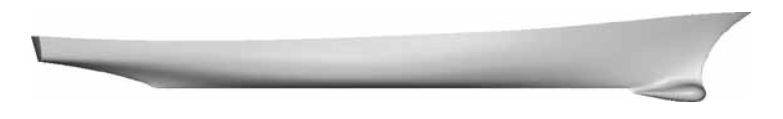
\includegraphics[width=1\textwidth]{DTMB.png}
    \caption{DTMB5415}
\end{figure}
\begin{figure}[ht]
    \centering
    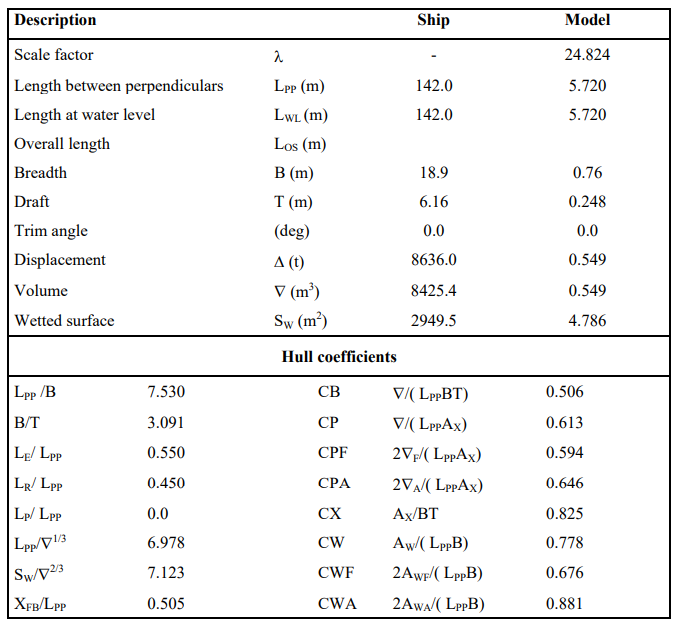
\includegraphics[width=1\textwidth]{DTMBsp.png}
    \caption{DTMB5415 Specifications\cite{olivieri2001}}
\end{figure}
\clearpage
\subsection{Domain \& Boundary Conditions}
The computational domain of this work is the reduced version of the Vaibhav's domain which was described in section 9.2.1 in \cite{joshi2018} as shown in figure 3. 
\begin{figure}[ht]
    \centering
    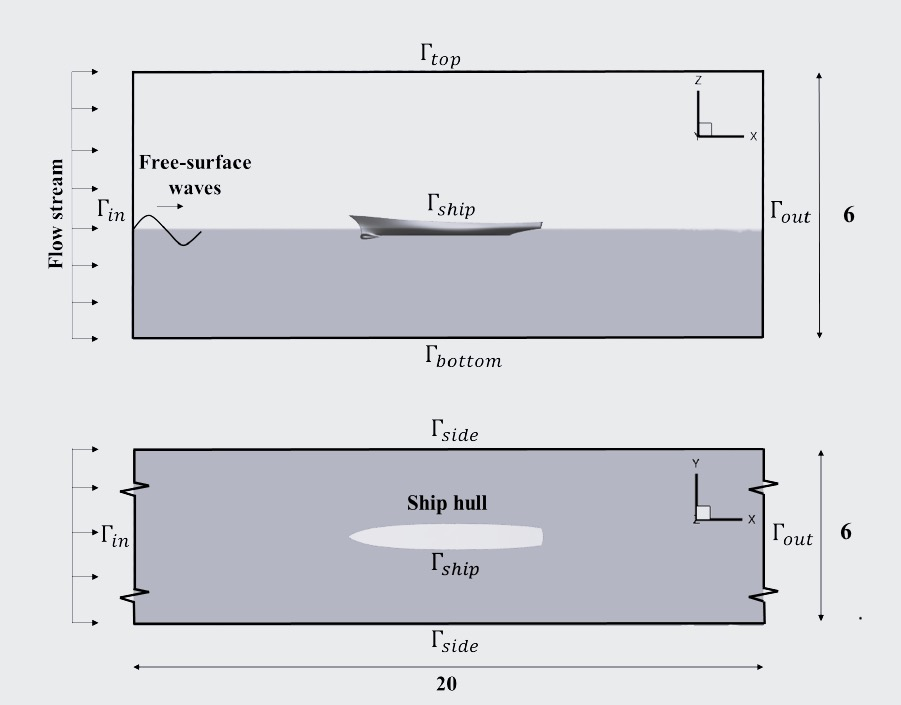
\includegraphics[width=1\textwidth]{Domain.jpg}
    \caption{DTMB5415 Specifications}
\end{figure}
The boundaries \(\Gamma_{\text{in}}\) and \(\Gamma_{\text{out}}\) shown in figure 3 denote the inlet 
and outlet. The inlet boundary is exposed to an incoming free-surface wave. 
%And the wave is described by
%\begin{align}
%u &= U_{\infty } + \frac{\pi H_w}{T_w} \cosh \left( k_w (z + h) \right) \left( \sinh (k_w h) \right)^{-1} \cos \left( k_w x - \frac{2 \pi}{T_w} t \right) \\
%v &= 0 \\
%w &= \frac{\pi H_w}{T_w} \sinh \left( k_w (z + h) \right) \left( \sinh (k_w h) \right)^{-1} \sin \left( k_w x - \frac{2 \pi}{T_w} t \right) \\
%\eta &= \frac{H_w}{2} \cos \left( k_w x - \frac{2 \pi}{T_w} t \right) \\
%\phi &= - \tanh \left( \frac{z - \eta}{\sqrt{2} \epsilon} \right)
%\end{align}
%where \(\mathbf{u}_f = (u, v, w)\) represents the fluid velocity components. \(U_1\) is the 
%freestream current velocity. \(H_w\), \(T_w\), and \(k_w\) denote the height, time period, and 
%wavenumber of the incoming linear waves, respectively. \(h\) is the water depth, and \(\eta\) is 
%the fluid-fluid interface profile.
%Detail of the wave will be discussed later. 
No condition is applied at the outlet boundary, the reason will be explained in section 3.5. 
Slip and no-slip boundary conditions are satisfied at the sides \(\Gamma_{\text{side}}\) and the 
ship hull surface \(\Gamma_{\text{ship}}\), respectively. An atmospheric condition is satisfied 
at \(\Gamma_{\text{top}}\) with a no-slip condition at \(\Gamma_{\text{bottom}}\).

\clearpage
\subsection{Mesh}
The mesh for the computational domain discussed in the previous section is constructed in Gmsh.
Note that for better view, only 2D mesh is presented below. A 3D view is provided in the Appendix 
section.
\begin{figure}[ht]
    \centering
    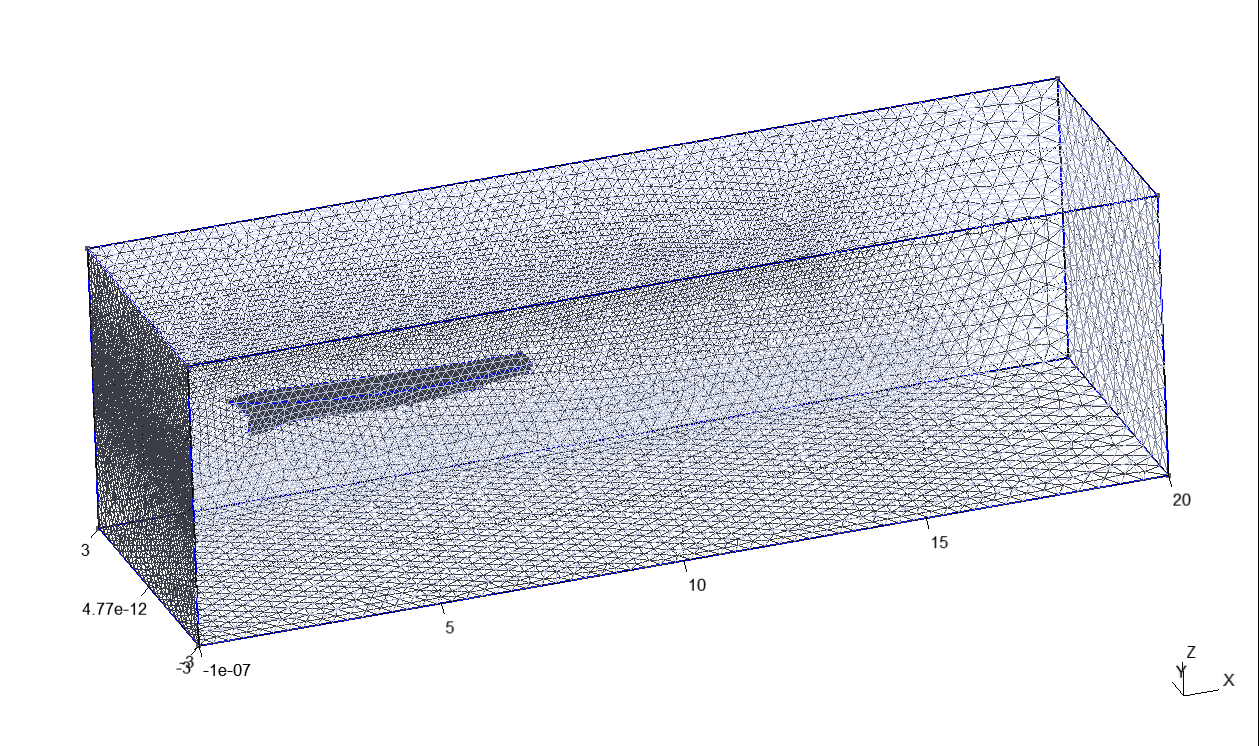
\includegraphics[width=0.6\textwidth]{Mesh_1.png}
    \caption{Mesh of the Domain}

\end{figure}
\begin{figure}[ht]
    \centering
    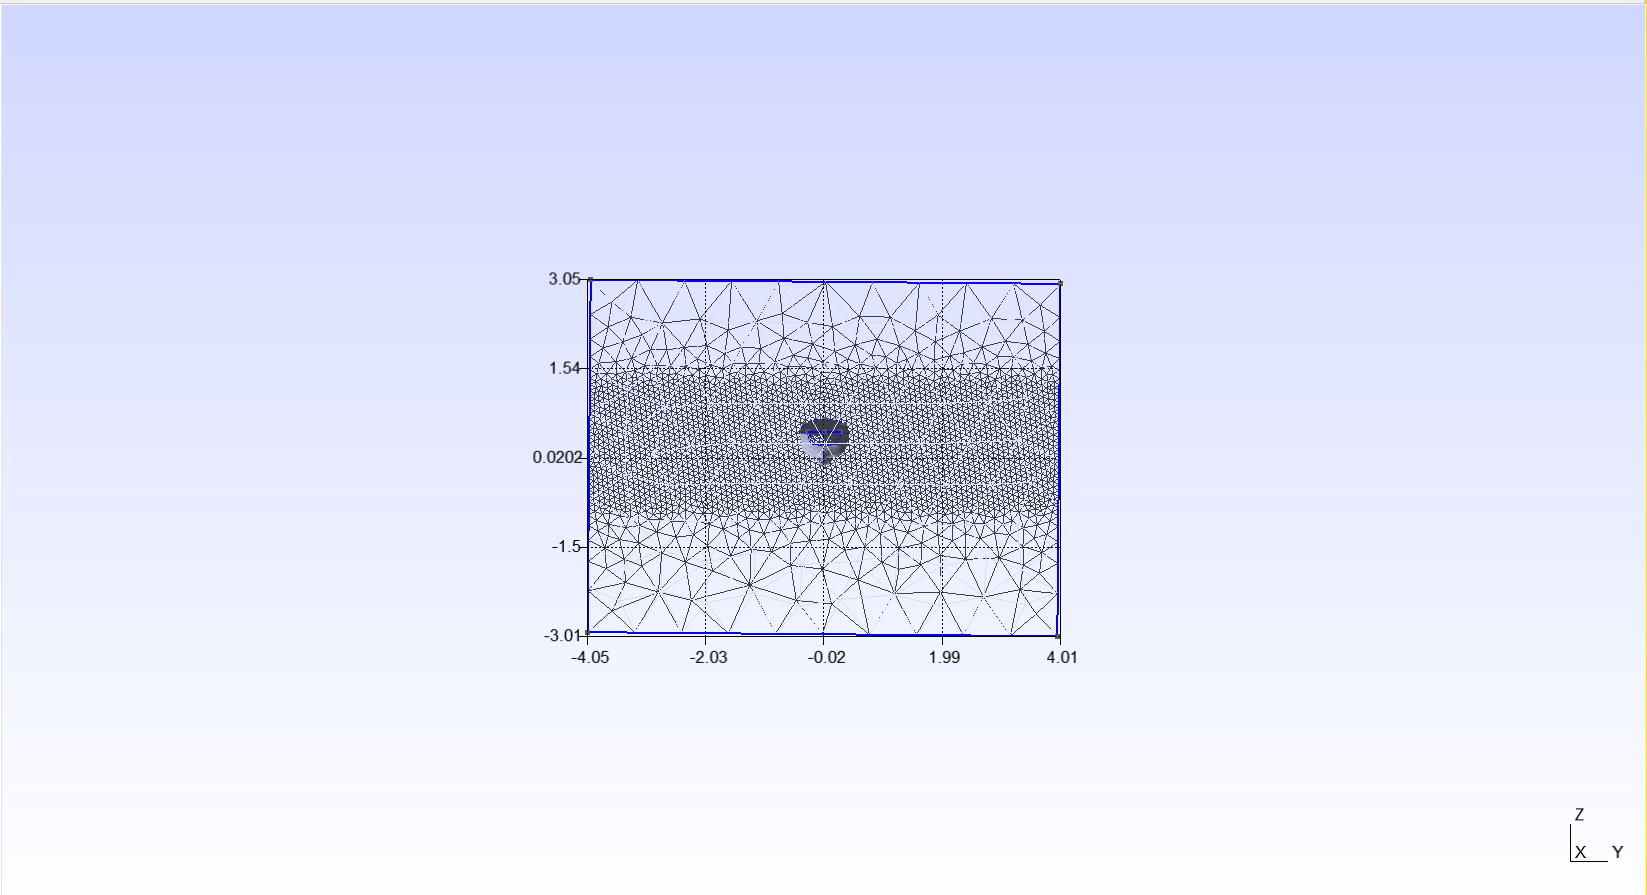
\includegraphics[width=0.9\textwidth]{Mesh_2.png}
    \caption{Front View of the Mesh}
\end{figure}

\begin{figure}[ht]
    \centering
    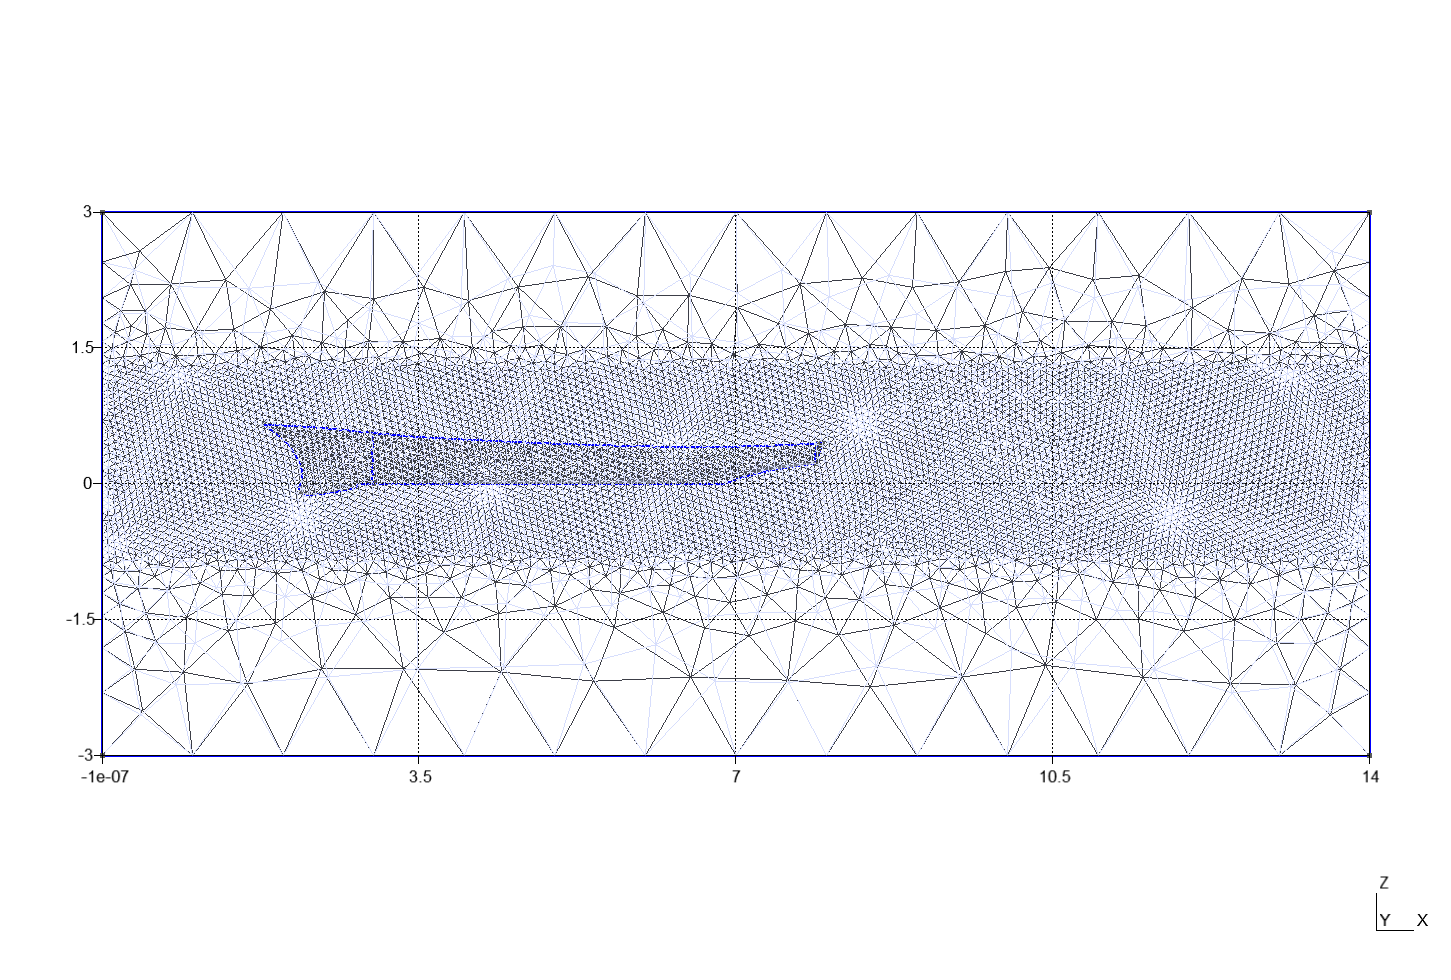
\includegraphics[width=0.9\textwidth]{Mesh_3.png}
    \caption{Side View of the Mesh}
\end{figure}

\begin{figure}[ht]
    \centering
    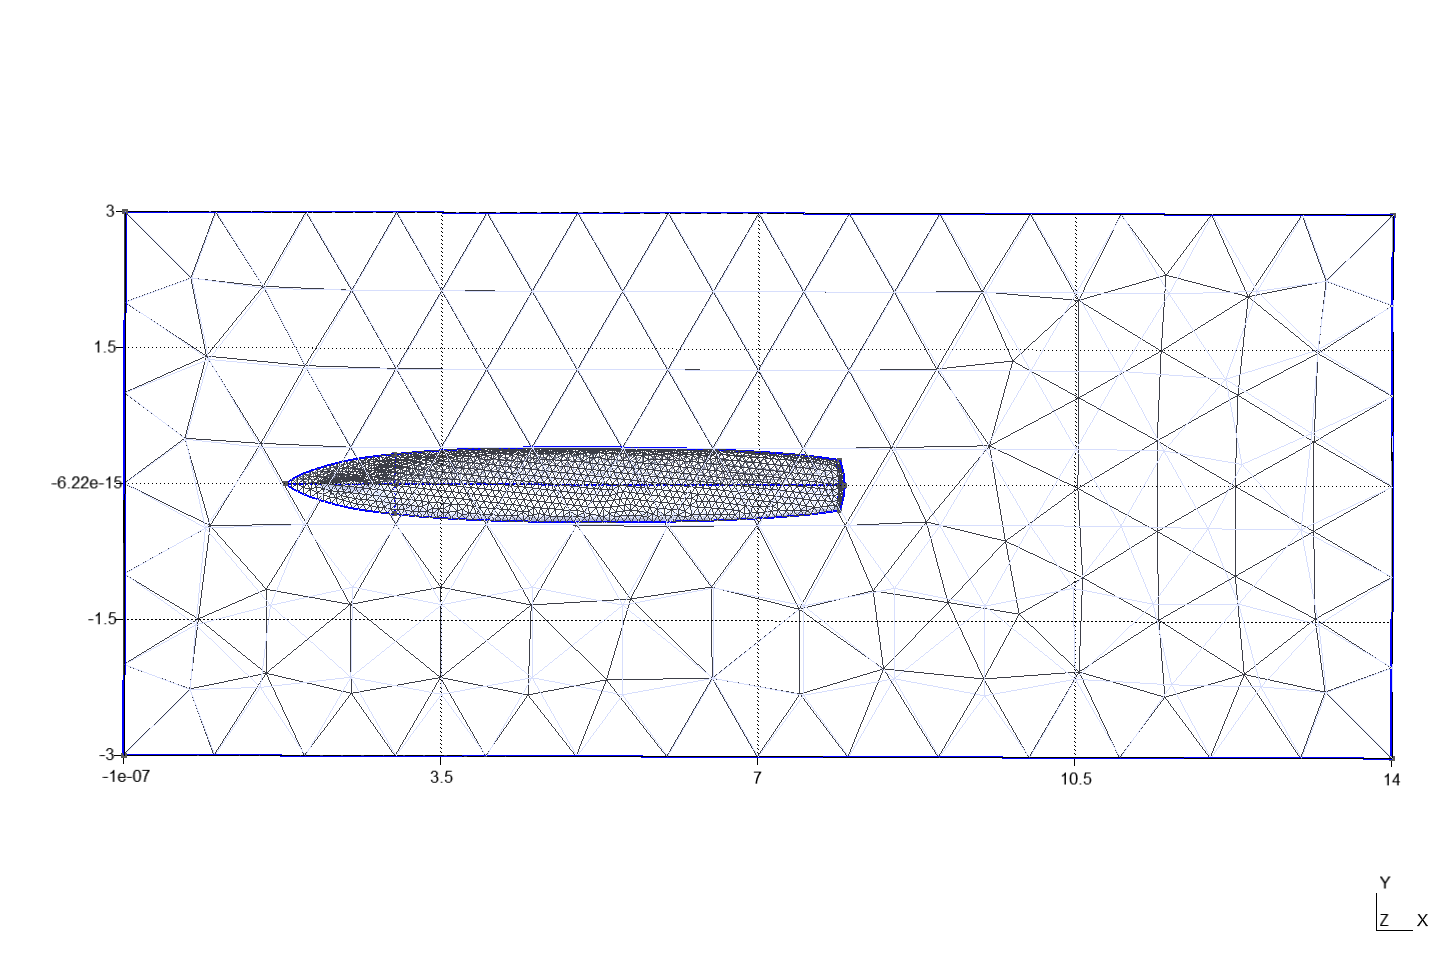
\includegraphics[width=0.9\textwidth]{Mesh_4.png}
    \caption{Top View of the Mesh}
\end{figure}
\clearpage
\subsection{Mesh Statistics}
Mesh details are shown in figure 8.
\begin{figure}[ht]
    \centering
    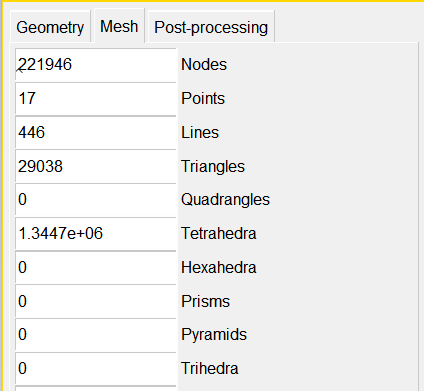
\includegraphics[width=0.5\textwidth]{MS.png}
    \caption{Mesh Statistics}
\end{figure}
\subsection{SIMFLOW Simulation Configuration}
The side boundaries are modeled with slip boundary conditions, while no-slip conditions are satisfied at the bottom and on the ship's surface. An atmospheric condition of \( p = 0 \) is satisfied at the top boundary. The physical properties of water and air are used for the two fluid phases, i.e., \( \rho_f^1 = 1000 \), \( \nu_f^1 = 1.002 \times 10^{-3} \), \( \rho_f^2 = 1.225 \), and \( \nu_f^2 = 1.983 \times 10^{-5} \). The acceleration due to gravity is \( g = (0, 0, -9.81) \).% For modeling incoming turbulence, the eddy viscosity at the inlet boundary is \( \tilde{\nu} = 5 \nu_f^1 / \rho_f^1 \).

Based on the given data of the DTMB 5415 ship model in section 3.1, the following non-dimensional numbers are employed, where \( V_{disp} \) is the volume of the displaced fluid at equilibrium. All variables are non-dimensionalized using the reference length \( L_{pp} \) and the freestream velocity \( U_1 \):
\begin{align*}
    Re &= \frac{\rho_f^1 U_1 L_{pp}}{\nu_f^1} = 1.069 \times 10^7 \\
    \rho^* &= \frac{\rho_f^1}{\rho_f^2} = 816 \\
    m^* &= \frac{m_s}{\rho_f^1 V_{disp}} = 1 \\
    \nu^* &= \frac{\nu_f^1}{\nu_f^2} = 50 \\
    Fr &= \frac{U_1}{\sqrt{g L_{pp}}} = 0.25
\end{align*}
At the inlet, a wave is generated with such parameters shown in table 1. \(\mathbf{u}_f = (u, v, w)\) represents the fluid velocity components. \(U_{u\infty}\) is the 
freestream current velocity. \(H_w\), \(T_w\), and \(k_w\) denote the height, time period, and 
wavenumber of the incoming wave.
\begin{table}[ht]
    \caption{Wave Conditions}
    \centering
    \begin{tabular}{|c|c|c|c|}
        \hline
        Parameters & Non-dimensional Value &Value & Unit\\
        \hline   
        $H_w$ & \(\frac{H_w}{L_{pp}} = 0.056\) &0.32032 & m \\
        $k_w$ & \(k_w = \frac{2\pi}{L_{pp}}\) &1.0845 & m\\
        $\lambda_w$ & \(k_w = \frac{L_{pp}}{2\pi}\) &0.91 & m\\
        $T_w$ & \(\frac{T_w U_1}{L_{pp}} = 0.629\) &1.929 & m \\
        \hline
    \end{tabular}
\end{table}

Moreover, the simualtion is configured by non-dimensional time step size of \(\Delta t \frac{U_1}{L_{pp}} = 3.27 \times 10^{-3}\) and a total of 2,400 time steps.


\section{Result}
\section{Discussion}
As a seciton of the HARP project, this work facilitates developing innovative tools for predicting underwater vessel noise during the design phase. It will identify potential noise sources, such as on-board machinery and propeller noise. Enhanced design models are anticipated to assist the industry in adopting `quiet' technologies for the next generation of ships, ensuring they maintain safety, productivity, and environmental performance.
\section{Future Work}
This work has only completed the first step of the scope stated in the methodology section. The future work is to replace the DTMB ship model with BURNSi model and conduct
test using the set-up mentioned above.
\section{Conclusion}



\section{Reference}
\begin{thebibliography}{99}
    \bibitem{joshi2018}
    Vaibhav Joshi, \emph{Variational Methods and Applications for Turbulent Single and Two-Phase Fluid-Structure Interaction}, ScholarBank@NUS Repository, 2018.

    \bibitem{olivieri2001}
    A. Olivieri, F. Pistani, A. Avanzini, F. Stern, and R. Penna, \emph{Towing tank experiments of resistance, sinkage and trim, boundary layer, wake, and free surface flow around a naval combatant INSEAN 2340 model}, IIHR Technical Report No. 421, 2001.
    
    \bibitem{kendrick2019}
    A. Kendrick and R. Terweij, \emph{Ship Underwater Radiated Noise}, Report 368-000-01, Rev 5, Vard Marine Inc., 08 July 2019.
   
    
    
    
\end{thebibliography}

\section{Appendix}
\subsection{DTMB 5415 Specifications}
\begin{table}[h!]
    \centering
    \begin{tabular}{|c|c|c|c|c|c|}
        \hline
        & \textbf{Full-Scale} & \textbf{\textcolor{blue}{MARIN}} & \textbf{\textcolor{blue}{INSEAN}} & \textbf{\textcolor{blue}{IIHR}} &\\ \hline
        \textbf{\textcolor{blue}{Lpp (m)}} & 142.00 & 4.002 & 4.002 & 5.719 & 3.048 \\ \hline
        \textbf{\textcolor{blue}{Lwl (m)}} & 142.18 & 4.007 & 4.008 & 5.726 & 3.052 \\ \hline
        \textbf{\textcolor{blue}{Bwl (m)}} & 19.06 & 0.537 & \textcolor{green}{0.538} & 0.768 & 0.409 \\ \hline
        \textbf{\textcolor{blue}{T (m)}} & 6.15 & 0.173 & \textcolor{green}{0.172} & 0.248 & 0.132 \\ \hline
        \textbf{\textcolor{blue}{Displacement (m\(^3\))}} & 8424.4 & 0.189 & \textcolor{green}{0.188} & 0.554 & 0.0826 \\ \hline
        \textbf{\textcolor{blue}{S w/o rudder (m\(^2\))}} & 2972.6 & 2.361 & \textcolor{green}{2.424} & TBD & TBD \\ \hline
        \textbf{\textcolor{blue}{CB}} & 0.507 & 0.507 & 0.507 & 0.506 & TBD \\ \hline
        \textbf{\textcolor{blue}{CM}} & 0.821 & 0.821 & 0.821 & 0.821 & 0.821 \\ \hline
        \textbf{\textcolor{blue}{LCB (\%Lpp), fwd+}} & -0.683 & -0.683 & \textcolor{green}{-0.652} & \textcolor{green}{-0.652} & TBD \\ \hline
    \end{tabular}
    \caption{Main particulars of the ship model}
\end{table}
\subsection{3D Mesh}
\begin{figure}[ht]
    \centering
    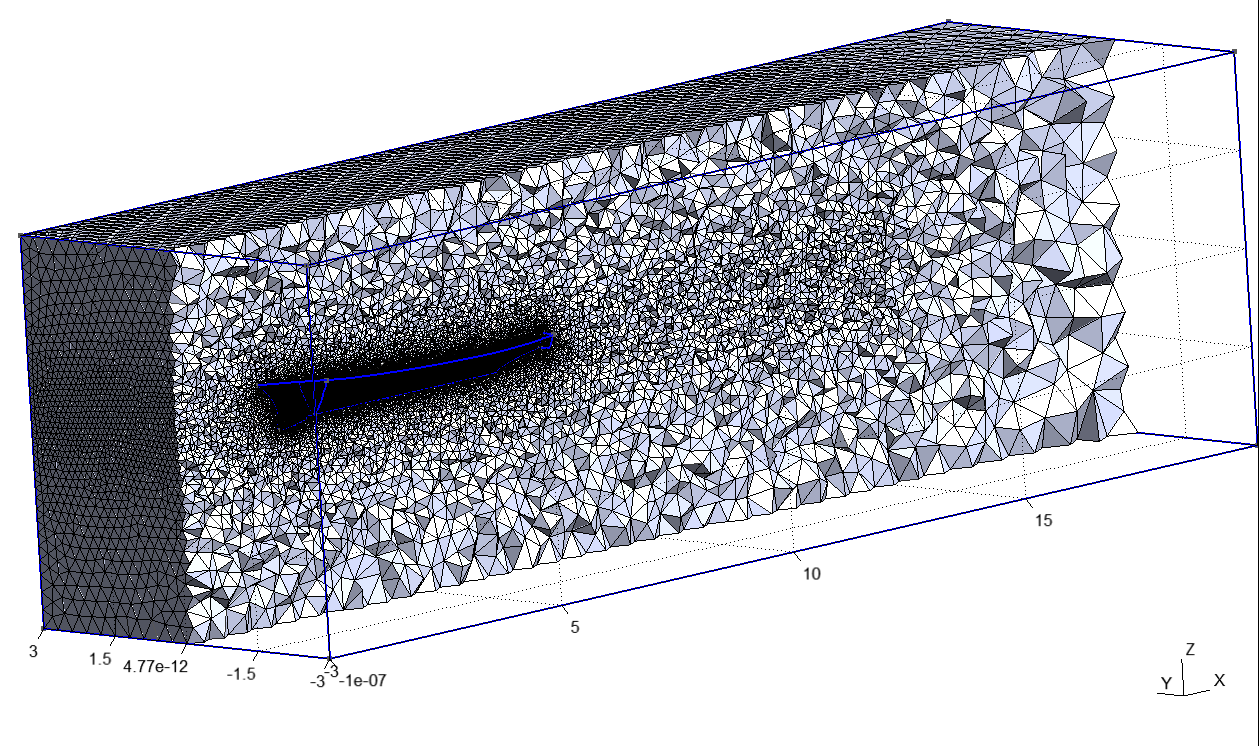
\includegraphics[width=1\textwidth]{Mesh_3D.png}
    \caption{3D Mesh}
\end{figure}

\end{document}